\chapter{QHashIterator}

template <typename Key, typename T> class QHashIterator

QHashIterator 类为 QHash 和 QMultiHash 提供 Java 风格的常量迭代器。更
多内容...

\begin{tabular}{|r|l|}
	\hline
头文件: &	\#include <QHashIterator>\\
\hline
qmake: &	QT += core\\
	\hline
\end{tabular}

\begin{compactitem}[\arr]
\item 所有成员列表,包括继承的成员
\item 废弃的成员
\end{compactitem}

\splitLine

\section{公共成员函数}

\begin{tabular}{|l|l|}
\hline
类型	&函数名\\
\hline
 	& QHashIterator(const QHash<Key, T> \&hash)\\
\hline
QHashIterator<Key, T> \& &	operator=(const QHash<Key, T> \&container)\\
\hline
bool &	findNext(const T \&value)\\
\hline
bool &	hasNext() const\\
\hline
const Key \& &	key() const\\
\hline
QHashIterator::Item &	next()\\
\hline
QHashIterator::Item &	peekNext() const\\
\hline
void &	toBack()\\
\hline
void &	toFront()\\
\hline
const T \& 	&value() const\\
\hline
\end{tabular}

\splitLine

\section{详细描述}

QHash 同时提供 Java 风格迭代器 和 STL 风格迭代器。Java 风格迭代器比 STL 风格迭代器更高级,更容易使用;同时也略微低效。

QHashIterator<Key, T> 用来遍历 QHash (或 QMultiHash)。如果想在遍历时修改哈希表,要使用 QMutableHashIterator。

QHashIterator 构造函数接受 QHash 作为参数。构造后,迭代器位于哈希表的最开始位置(第一个元素之前)。下面的例子演示如何顺序遍历所有元素:

\begin{lstlisting}[language=C++]
QHash<int, QWidget *> hash;
...
QHashIterator<int, QWidget *> i(hash);
while (i.hasNext()) {
    i.next();
    qDebug() << i.key() << ": " << i.value();
}
\end{lstlisting}

next() 函数返回哈希表中的下一个元素并将迭代器前移。key() 和 value() 函数返回跳过的最后一个元素的键和值。

与 STL 风格迭代器不同,Java 风格迭代器指向元素之间而不是直接指向元素。
第一次调用 next() 前移迭代器到第一个和第二个元素\emph{之间}的位置,并返回第一
个元素;第二次调用 next() 前移迭代器到第二个和第三个元素之间的位置;以
此类推。


\begin{figure}[hbt!]  
	\centering
    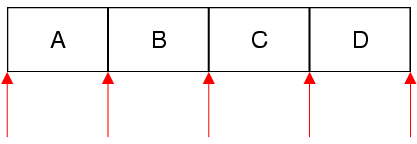
\includegraphics[width=0.5\textwidth]{qhash-iterator}
	%\caption{model index}
\end{figure}

如果想查找特定值的所有实例,循环使用 findNext()。例如:

\begin{lstlisting}[language=C++]
QHashIterator<int, QWidget *> i(hash);
while (i.findNext(widget)) {
    qDebug() << "Found widget  " << widget << " under key "
             << i.key();
}
\end{lstlisting}

同一哈希表可以使用多个迭代器。如果在 QHashIterator处于活动状态时修改哈希表,QHashIterator 将继续在原哈希表上遍历,而忽略修改后的副本。


\begin{seeAlso}
QMutableHashIterator 和 QHash::const\_iterator。
\end{seeAlso}

\splitLine

\section{成员函数文档}

bool QHashIterator::findNext(const T \emph{\&value})

从当前迭代器位置开始向前查找值 \emph{value}。如果找到值为 \emph{value} 的键值对,返回 \hl{true};否则返回 \hl{false}。

调用该函数后,如果找到值 \emph{value},迭代器将被移动到匹配元素的后面;否则,
迭代器将被移动到容器的末端。

const Key \&QHashIterator::key() const

调用遍历函数((next(),findNext())后,该函数返回跳过的最后一个元素的键。

\begin{seeAlso}
value()。
\end{seeAlso}

bool QHashIterator::hasNext() const

如果该迭代器后面至少有一个元素,返回 \hl{true},即该迭代器不在容器的末端;否则返回 \hl{false}。


\begin{seeAlso}
next()。
\end{seeAlso}


void QHashIterator::toBack()

将迭代器移动到容器的末端(最后一个元素之后)。



\begin{seeAlso}
toFront()。
\end{seeAlso}


void QHashIterator::toFront()

将迭代器移动到容器的前端(第一个元素之前)。




\begin{seeAlso}
toBack() 和 next()。
\end{seeAlso}


QHashIterator<Key, T> \&QHashIterator::operator=(const QHash<Key, T> \emph{\&container})

将迭代器关联到 \emph{container} 来遍历哈希表。迭代器将被移动到哈希表的前端(第一个元素之前)。



\begin{seeAlso}
toFront() 和 toBack()。
\end{seeAlso}


QHashIterator::QHashIterator(const QHash<Key, T> \emph{\&hash})

构造一个迭代器来遍历 \emph{hash}。迭代器将被移动到哈希表的前端(第一个元素之前)。


\begin{seeAlso}
operator=()。
\end{seeAlso}


QHashIterator::Item QHashIterator::next()

返回下一个元素并将迭代器向前移动一个位置。

对返回值调用 key() 获取元素的键,调用 value() 获取元素的值。

对位于容器末端的迭代器调用该函数将导致未定义结果。



\begin{seeAlso}
hasNext() 和 peekNext()。
\end{seeAlso}

QHashIterator::Item QHashIterator::peekNext() const

不移动迭代器而返回下一个元素。

对返回值调用 key() 获取元素的键,调用 value() 获取元素的值。

对位于容器末端的迭代器调用该函数将导致未定义结果。


\begin{seeAlso}
hasNext() 和 next()。
\end{seeAlso}

const T \&QHashIterator::value() const

调用遍历函数(next(),findNext())后,该函数返回跳过的最后一个元素的值。

\begin{seeAlso}
key()。
\end{seeAlso}

%%% Local Variables:
%%% mode: latex
%%% TeX-master: "../../master"
%%% End: